% ------------------------------------------------------------
% Three columns
% ------------------------------------------------------------

\begin{columns}[t,totalwidth=\textwidth]

% First column
\begin{column}{0.31\textwidth}

\begin{block} {Atom and molecules}
  A \cemph{molecule} is a combinatorial datum encoding the shape of a higher categorical pasting diagram.
  A molecule \( U \):
  \begin{itemize}
    \item is an \cemph{oriented} and graded poset; 
    \item has for each \( \a \in \set{-, +} \) and \( n \in \nat \), a \cemph{input/output \( n \)\nbd boundary}, \( \bd{n}{\a} U \), which is a closed subset of \( U \).
  \end{itemize}
  Molecule can be \cemph{pasted} together: given \( U \), \( V \), and \( n \in \nat \), if \( \bd{i}{+} U \cong \bd{i}{-} V \), then the pushout
  \begin{center}
    \begin{tikzcd}
      {\bd{i}{+} U \cong \bd{i}{-} V} & V \\
      U & {U \cp{k} V}
      \arrow[""{name=0, anchor=center, inner sep=0}, hook, from=1-1, to=1-2]
      \arrow[from=1-1, to=2-1]
      \arrow[from=1-2, to=2-2]
      \arrow[hook, from=2-1, to=2-2]
      \arrow["\lrcorner"{anchor=center, pos=0.125, rotate=180}, draw=none, from=2-2, to=0]
    \end{tikzcd}
  \end{center}
  is a molecule.
  Pasting and boundary of molecules satisfy all the axioms of strict \( \omega \)\nbd categories, and even some \gemph{higher-exchange laws} in dimension \( \geq 4 \).
  An \cemph{atom} is a molecule with a greatest cell.
\end{block}

\vspace{-1em}
\begin{block}{Directed complexes}
    A \cemph{directed complex} \( X \) is a presheaf over the category of atoms.
    It is the combinatorial data to construct a \remph{positive} and \remph{regular} polygraphs:
    \begin{center}
      \begin{tikzcd}
        {\coprod\limits_{u \in \cls S_n} \bd{}{} U} & {\coprod\limits_{u \in \cls S_n} U} \\
        {X_{n - 1}} & {X_n,}
        \arrow[""{name=0, anchor=center, inner sep=0}, hook, from=1-1, to=1-2]
        \arrow["{(\bd{}{}u)_{u \in \cls S_n}}"', from=1-1, to=2-1]
        \arrow["{(u)_{u \in \cls S_n}}", from=1-2, to=2-2]
        \arrow[hook, from=2-1, to=2-2]
        \arrow["\lrcorner"{anchor=center, pos=0.125, rotate=180}, draw=none, from=2-2, to=0]
      \end{tikzcd}
    \end{center}
    There is a construction \( \molecin{X} \) that produces the strict \( \omega \)\nbd category of \remph{molecules in \( X \)}.
    \begin{itemize}
      \item If \( X \) is a graph, \( \molecin{X} \) is the free category on \( X \);
      \item If \( X \) is the \( n \)\nbd dimensional simplex, then \( \molecin{X} \) is the \( n \)\nbd oriental.  
    \end{itemize}
    \red{\uline{Theorem 1.}} under a general acyclicity condition on its molecules, \( \molecin{X} \) is a polygraph, and in fact, a \gemph{weak polygraph}.
\end{block}

\begin{block} {Operations}
  Atom, molecules, and directed complexes, support natively higher categorical operations:
  \begin{itemize}
    \item Gray product \( X \gray Y \),
    \item join \( X \join Y \),
    \item suspension \( \sus{X} \),
    \item duals \( \fun{D}_J X \), where \( J \subseteq \nat \).
  \end{itemize}
\end{block}
\end{column}

% Space between columns
\begin{column}{0.025\textwidth}
\end{column}

% Second column
\begin{column}{0.31\textwidth}

\begin{block}{Examples}

\begin{center}
  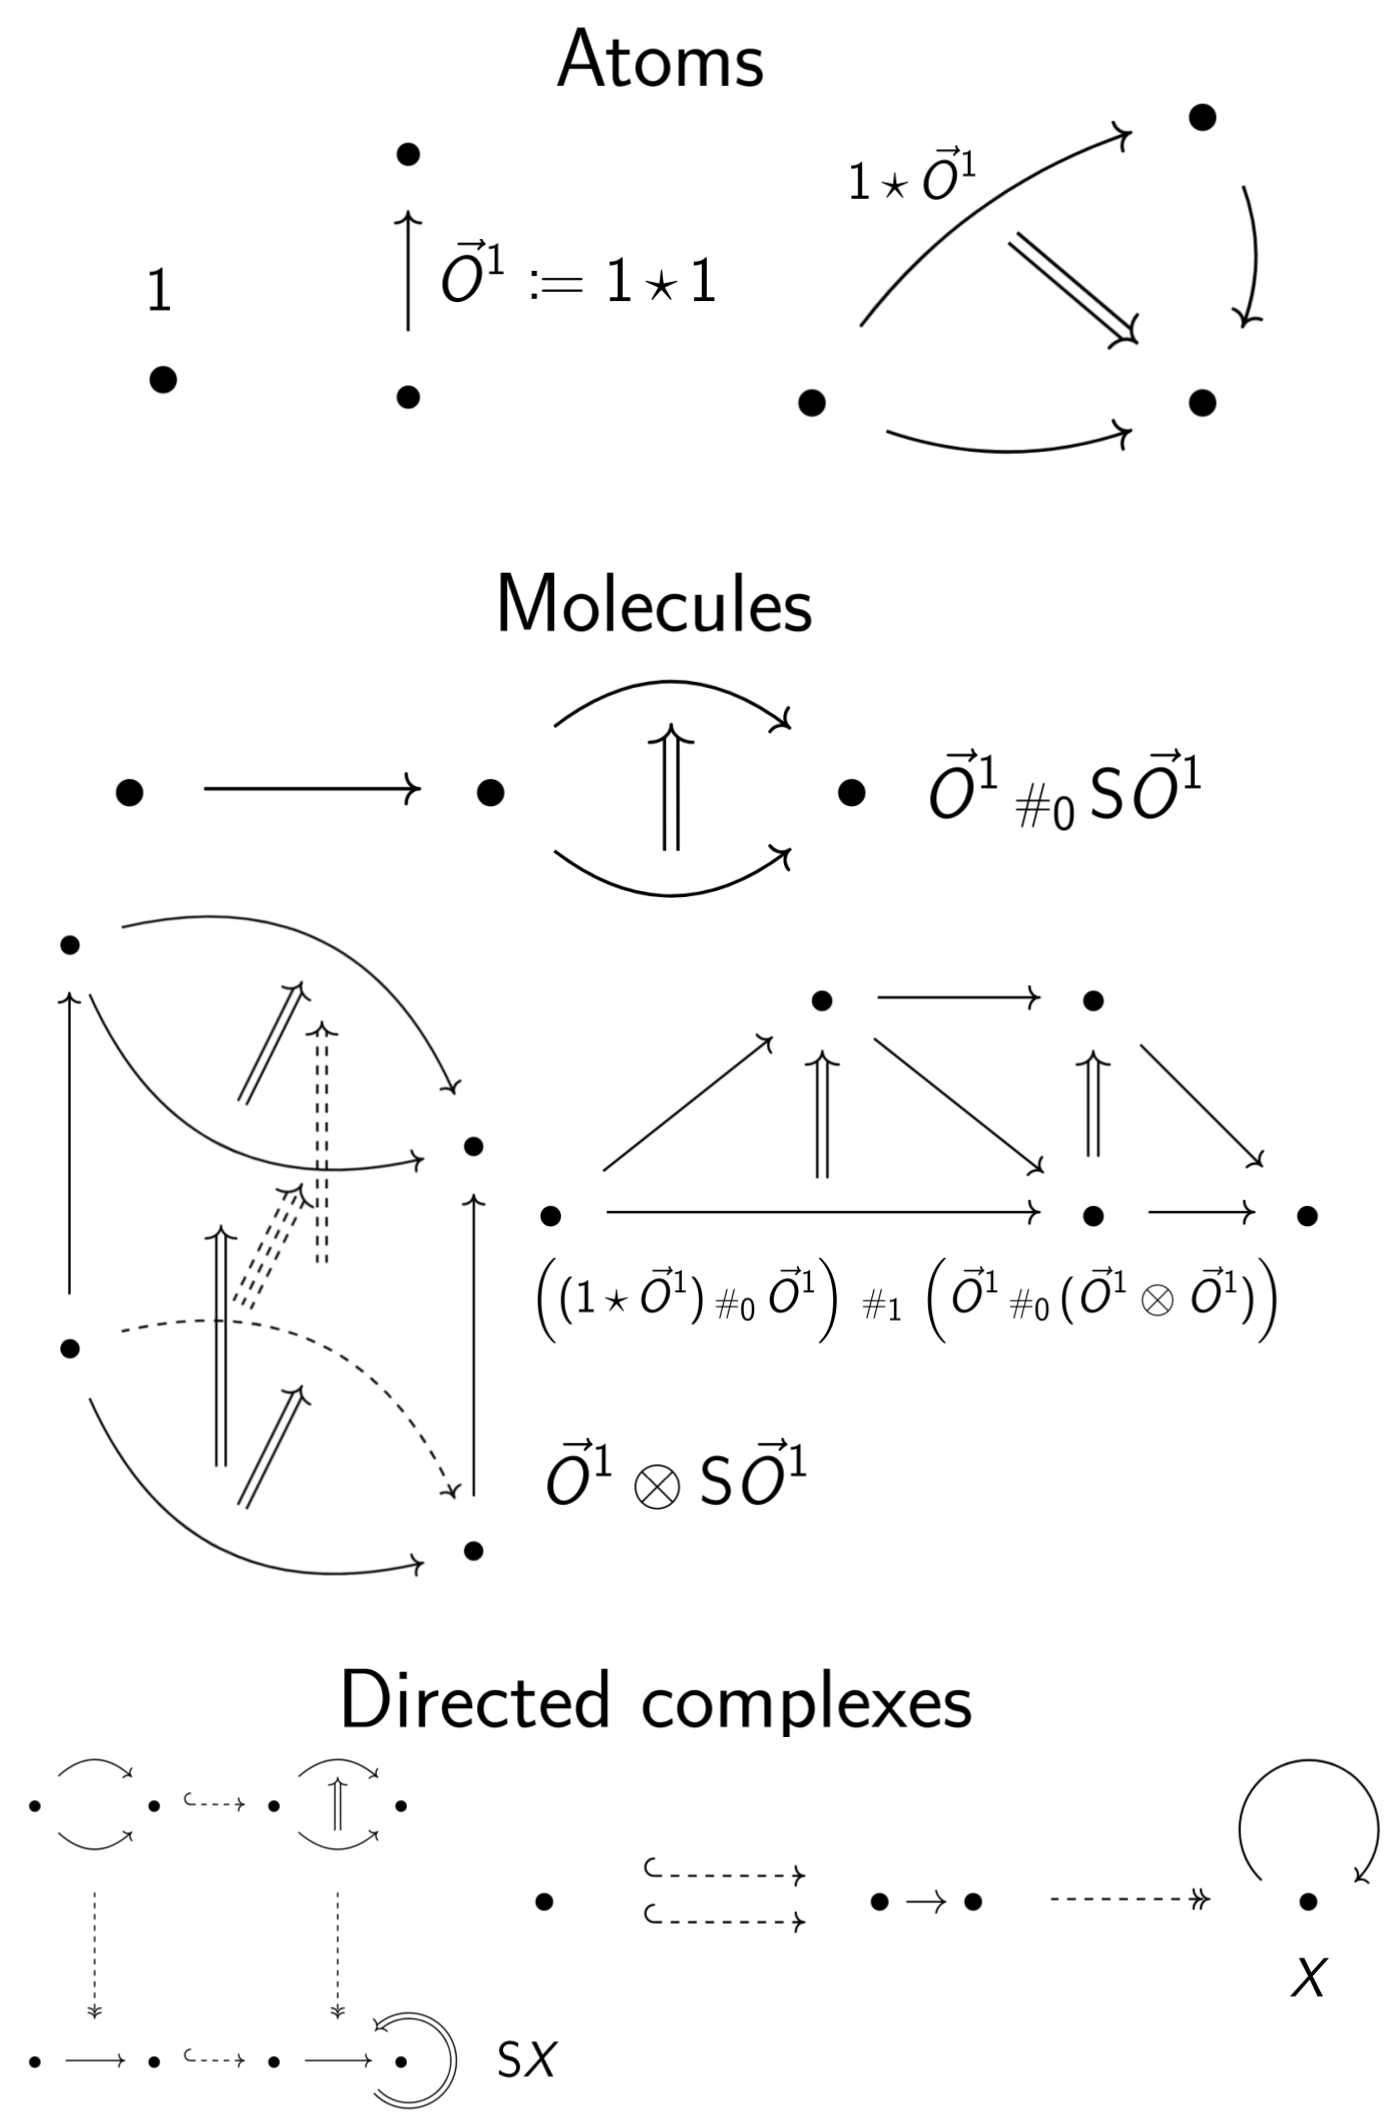
\includegraphics[scale=0.5]{img/exx.png}  
\end{center}
In the last example:
\begin{itemize}
  \item \( \molecin{X} = \fun{B}\nat\)
  \item \( X \) satisfies the acyclicity hypothesis\\ of \red{\uline{Theorem 1.}}
\end{itemize}
  %   {\Large Atoms} \\
%   \vspace{3em}
%   {\Large Molecules} \\
%   \vspace{3em}
%   {\Large Directed complexes} \\
%   \begin{equation*}
%     \pt\quad \globe{1} \eqdef \pt \join \pt\quad \pt \join \globe{1}\quad \globe{1} \cp{0} \sus{\globe{1}}
%   \end{equation*}
%   \begin{equation*}
%     \globe{1} \gray \sus{\globe{1}} \quad \left((\pt \join \globe{1}) \cp{0} \globe{1}\right) \cp{1} \left(\globe{1} \cp{0} (\globe{1} \gray \globe{1})\right)
%   \end{equation*}
%   \vspace{3em}
% \begin{equation*}
%   X \quad \molecin{X} = \fun{B}\nat \quad \sus{X}
% \end{equation*}
% \begin{itemize}
%   \item \( \molecin{X} = \fun{B}\nat\)
%   \item \( X \) satisfies the acyclicity hypothesis\\ of \red{\uline{Theorem 1.}}
% \end{itemize}
\end{block}
\end{column}

% Space between columns
\begin{column}{0.025\textwidth}
\end{column}

% Third columné
\begin{column}{0.31\textwidth}

\begin{block}{Diagrammatic \( (\infty, n) \)\nbd categories}
  Directed complexes may be used in several ways to construct models of \( (0, n) \) and \( (\infty, n) \)\nbd categories:
  \begin{enumerate}
    \item as Segal-sheaves over the \( \molecin{X} \)'s and \remph{strict functors}; 
    \item as presheaves over the atoms and \remph{cellular} strict functors between them;
    A localisation enforces the existence of \cemph{weak composites}.
  \end{enumerate}
  This matches the following two perspective on standard \( (\infty, n) \)\nbd categories as
  \begin{itemize}
    \item Segal-sheaves over the theta's and strict functors;
    \item presheaves over the (marked) orientals and cellular strict functors (i.e. over the marked simplex category).
  \end{itemize}
  \red{\uline{Theorem.}} point \remph{1.} is a localisation of the \( (\infty, n) \)\nbd categories at the higher-exchanges, which does nothing when \( n \le 3 \). \\
  \red{\uline{Conjecture.}} point \remph{1.} and \remph{2.} present the same model of higher-categories.
\end{block}

\begin{block} {Features of the diagrammatic models}
  \begin{itemize}
    \item Very strong \remph{pasting theorems};
    \item \remph{Semi-strictification:} marked directed complexes may be used to two \red{equivalent} model:
    \begin{enumerate}
      \item one where composition is witnessed by \gemph{the existence} of weak composites;
      \item one where composition is \gemph{an operation} satisfying strict associativity and exchange; 
    \end{enumerate}
    In both cases, the unit are algebraic and weak.  
    \item Native support of \remph{higher categorical constructions}, no need to use different presentation.
    \item A rich algebra of \remph{weak units}.
    \item An overall feeling of a \remph{topologically sound alternative} to strict \( n \)\nbd categories
  \end{itemize}
\end{block}
\begin{block}{References}

\small

\begin{thebibliography}{9}

\bibitem{equivalences}
C.~Chanavat and A.~Hadzihasanovic,
\emph{Equivalences in diagrammatic sets},
\newblock Journal of Pure and Applied Algebra, 2026.

\bibitem{reference}
A.~Author,
\newblock \emph{Another reference},
\newblock Journal, year.

\end{thebibliography}

\end{block}

\end{column}

\end{columns}